\section{Road trip in Romania \cite{ai/book/Artificial-Intelligence-A-Modern-Approach/Russell-Norvig}}


\begin{figure}[H]
    \centering
    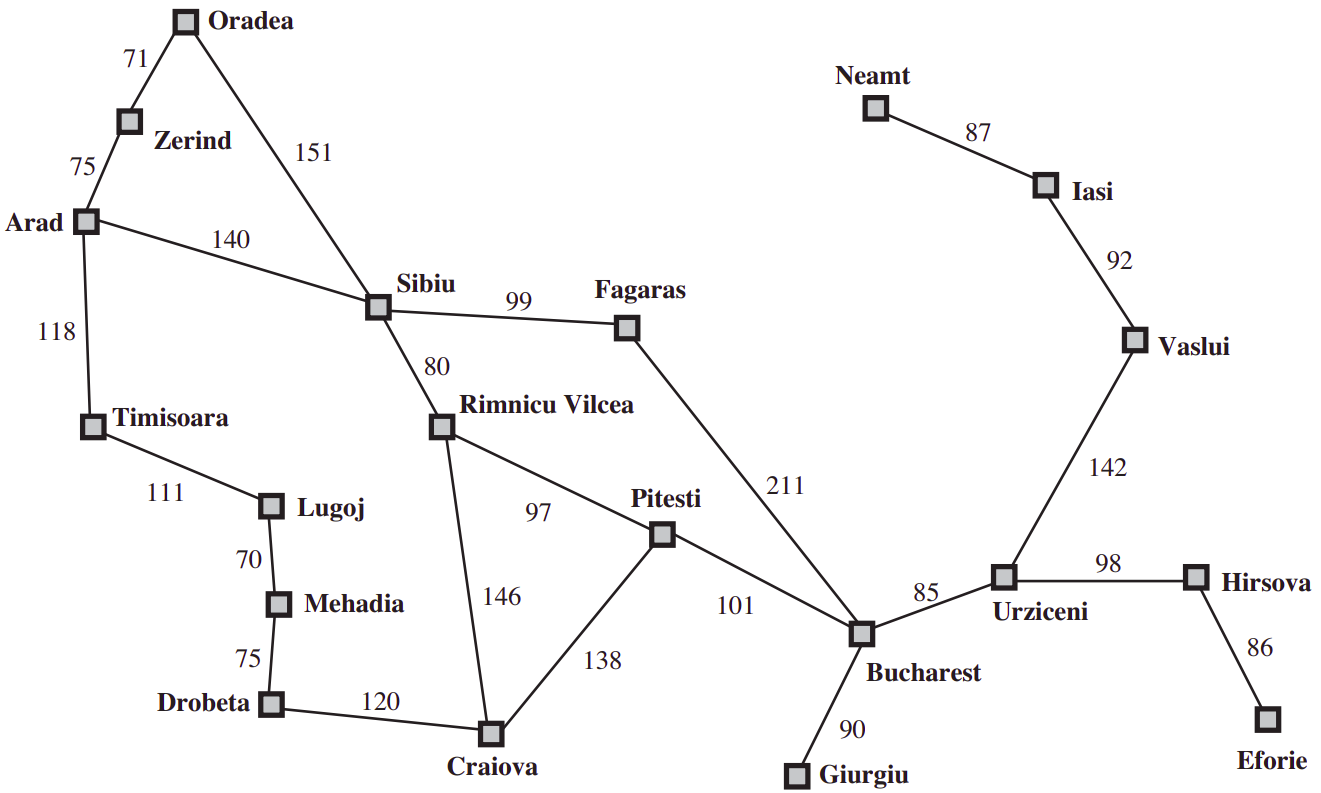
\includegraphics[
        width=\linewidth,
        height=8cm,
        keepaspectratio,
    ]{images/artificial-intelligence/examples/romania-map.png}
    \caption*{A simplified road map of part of Romania. \cite{ai/book/Artificial-Intelligence-A-Modern-Approach/Russell-Norvig}}
\end{figure}


\begin{figure}[H]
    \centering
    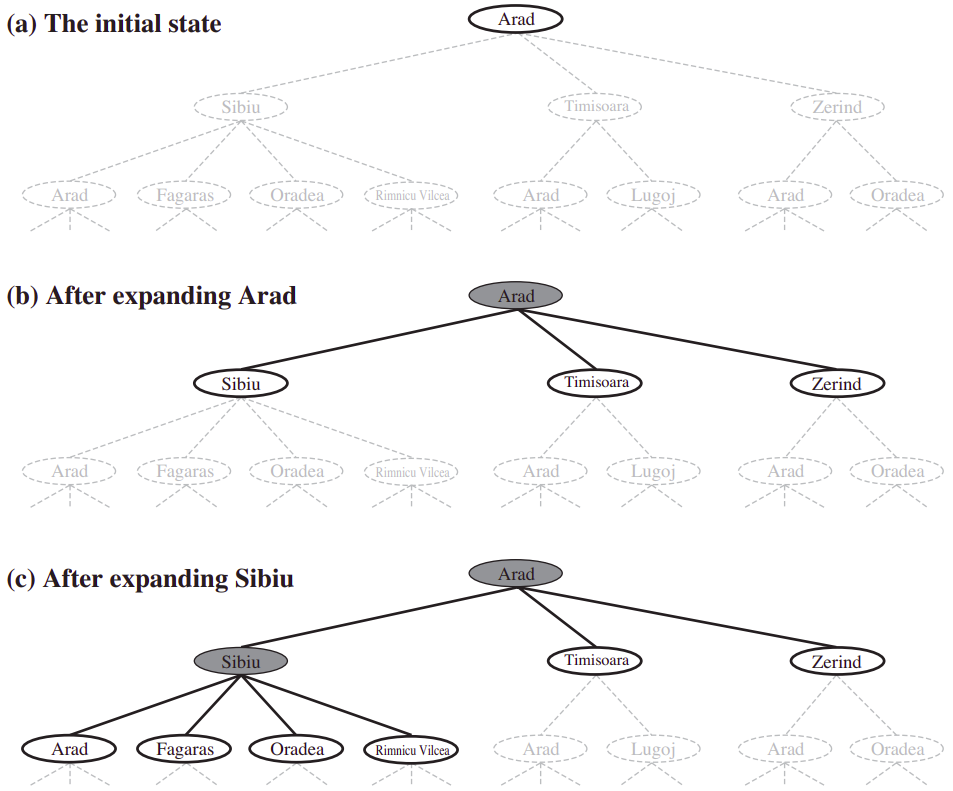
\includegraphics[
        width=\linewidth,
        height=10cm,
        keepaspectratio,
    ]{images/artificial-intelligence/examples/romania-search-tree.png}
    \caption*{Partial search trees for finding a route from Arad to Bucharest. Nodes that have been expanded are shaded; nodes that have been generated but not yet expanded are outlined in bold; nodes that have not yet been generated are shown in faint dashed lines. \cite{ai/book/Artificial-Intelligence-A-Modern-Approach/Russell-Norvig}}
\end{figure}



\begin{enumerate}[itemsep=0.2cm]
    \item we use the straight-line distance (SLD) heuristic
    \hfill \cite{ai/book/Artificial-Intelligence-A-Modern-Approach/Russell-Norvig}
\end{enumerate}


\vspace{0.5cm}

{\centering \textbf{Defining Problem \& State} \par}

\begin{lstlisting}[language=Python]
# src: {tgt: path_cost}
romania_map_graph = {
    "Arad": {"Timisoara": 118, "Sibiu": 140, "Zerind": 75},
    "Bucharest": {"Pitesti": 101, "Fagaras": 211, "Giurgiu": 90, "Urziceni": 85},
    "Craiova": {"Drobeta": 120, "Rimnicu Vilcea": 146, "Pitesti": 138},
    "Drobeta": {"Mehadia": 75, "Craiova": 120},
    "Eforie": {"Hirsova": 86},
    "Fagaras": {"Sibiu": 99, "Bucharest": 211},
    "Giurgiu": {"Bucharest": 90},
    "Hirsova": {"Urziceni": 98, "Eforie": 86},
    "Iasi": {"Vaslui": 92, "Neamt": 87},
    "Lugoj": {"Mehadia": 70, "Timisoara": 111},
    "Mehadia": {"Lugoj": 70, "Drobeta": 75},
    "Neamt": {"Iasi": 87},
    "Oradea": {"Zerind": 71, "Sibiu": 151},
    "Pitesti": {"Rimnicu Vilcea": 97, "Craiova": 138, "Bucharest": 101},
    "Rimnicu Vilcea": {"Sibiu": 80, "Pitesti": 97, "Craiova": 146},
    "Sibiu": {"Fagaras": 99, "Rimnicu Vilcea": 80, "Arad": 140, "Oradea": 151},
    "Timisoara": {"Arad": 118, "Lugoj": 111},
    "Urziceni": {"Bucharest": 85, "Vaslui": 142, "Hirsova": 98},
    "Vaslui": {"Urziceni": 142, "Iasi": 92},
    "Zerind": {"Arad": 75, "Oradea": 71},
}

heuristic_Bucharest = {
    "Arad": 366,
    "Bucharest": 0,
    "Craiova": 160,
    "Drobeta": 242,
    "Eforie": 161,
    "Fagaras": 176,
    "Giurgiu": 77,
    "Hirsova": 151,
    "Iasi": 226,
    "Lugoj": 244,
    "Mehadia": 241,
    "Neamt": 234,
    "Oradea": 380,
    "Pitesti": 100,
    "Rimnicu Vilcea": 193,
    "Sibiu": 253,
    "Timisoara": 329,
    "Urziceni": 80,
    "Vaslui": 199,
    "Zerind": 374,
}


class RomaniaState(State):
    def __init__(self, city: str) -> None:
        self.city = city

    def copy(self):
        return RomaniaState(self.city)
    
    def __str__(self):
        return f"<RomaniaState city={self.city}>"

    def __repr__(self):
        return str(self)
    
    def __eq__(self, __o):
        return self.city == __o.city

class RomaniaProblem(Problem):
    def __init__(self, initial_state: RomaniaState):
        super().__init__(initial_state)
    
    def goal_test(self, state: RomaniaState):
        return state.city == "Bucharest"
    
    def step_cost(self, state: RomaniaState, action: str, new_state: RomaniaState):
        return romania_map_graph[state.city][new_state.city]
    
    def heuristic(self, state: RomaniaState):
        return heuristic_Bucharest[state.city]
    
    def actions(self, state: RomaniaState):
        return sorted(romania_map_graph[state.city].keys())
    
    def result(self, state: RomaniaState, action: str):
        return RomaniaState(action)


initial_state = RomaniaState("Arad")
problem = RomaniaProblem(initial_state=initial_state)
\end{lstlisting}



{\centering \textbf{Solution using breadth\_first\_search} \par}

\begin{lstlisting}[language=Python]
path = breadth_first_search(problem)
print(path)

node = Node(initial_state, None, None, 0)
for e in path:
    new_node = child_node(problem, node, e)
    print(
        node.state.city.ljust(20), 
        new_node.state.city.ljust(20), 
        str(new_node.path_cost - node.path_cost).rjust(5), 
        str(new_node.path_cost).rjust(5)
    )
    node = new_node
\end{lstlisting}


{\centering \textbf{Solution using uniform\_cost\_search} \par}

\begin{lstlisting}[language=Python]
path = uniform_cost_search(problem)
print(path)

node = Node(initial_state, None, None, 0)
for e in path:
    new_node = child_node(problem, node, e)
    print(
        node.state.city.ljust(20), 
        new_node.state.city.ljust(20), 
        str(new_node.path_cost - node.path_cost).rjust(5), 
        str(new_node.path_cost).rjust(5)
    )
    node = new_node
\end{lstlisting}



{\centering \textbf{Solution using depth\_first\_search} \par}

\begin{lstlisting}[language=Python]
path = depth_first_search(problem)
print(path)

node = Node(initial_state, None, None, 0)
for e in path:
    new_node = child_node(problem, node, e)
    print(
        node.state.city.ljust(20), 
        new_node.state.city.ljust(20), 
        str(new_node.path_cost - node.path_cost).rjust(5), 
        str(new_node.path_cost).rjust(5)
    )
    node = new_node
\end{lstlisting}


{\centering \textbf{Solution using backtracking\_search} \par}

\begin{lstlisting}[language=Python]
path = backtracking_search(problem)
print(path)

node = Node(initial_state, None, None, 0)
for e in path:
    new_node = child_node(problem, node, e)
    print(
        node.state.city.ljust(20), 
        new_node.state.city.ljust(20), 
        str(new_node.path_cost - node.path_cost).rjust(5), 
        str(new_node.path_cost).rjust(5)
    )
    node = new_node
\end{lstlisting}



{\centering \textbf{Solution using depth\_limited\_search} \par}

\begin{lstlisting}[language=Python]
path = depth_limited_search(problem, 4)
print(path)

node = Node(initial_state, None, None, 0)
for e in path:
    new_node = child_node(problem, node, e)
    print(
        node.state.city.ljust(20), 
        new_node.state.city.ljust(20), 
        str(new_node.path_cost - node.path_cost).rjust(5), 
        str(new_node.path_cost).rjust(5)
    )
    node = new_node

print("\n")

path = depth_limited_search(problem, 2)
print(path)

if isinstance(path, list):
    node = Node(initial_state, None, None, 0)
    for e in path:
        new_node = child_node(problem, node, e)
        print(
            node.state.city.ljust(20), 
            new_node.state.city.ljust(20), 
            str(new_node.path_cost - node.path_cost).rjust(5), 
            str(new_node.path_cost).rjust(5)
        )
        node = new_node
\end{lstlisting}


{\centering \textbf{Solution using iterative\_deepening\_search} \par}

\begin{lstlisting}[language=Python]
path = iterative_deepening_search(problem)
print(path)

node = Node(initial_state, None, None, 0)
for e in path:
    new_node = child_node(problem, node, e)
    print(
        node.state.city.ljust(20), 
        new_node.state.city.ljust(20), 
        str(new_node.path_cost - node.path_cost).rjust(5), 
        str(new_node.path_cost).rjust(5)
    )
    node = new_node
\end{lstlisting}


{\centering \textbf{Solution using iterative\_lengthening\_search} \par}

\begin{lstlisting}[language=Python]
path = iterative_lengthening_search(problem)
print(path)

node = Node(initial_state, None, None, 0)
for e in path:
    new_node = child_node(problem, node, e)
    print(
        node.state.city.ljust(20), 
        new_node.state.city.ljust(20), 
        str(new_node.path_cost - node.path_cost).rjust(5), 
        str(new_node.path_cost).rjust(5)
    )
    node = new_node
\end{lstlisting}


{\centering \textbf{Solution using A* search} \par}

\begin{figure}[H]
    \centering
    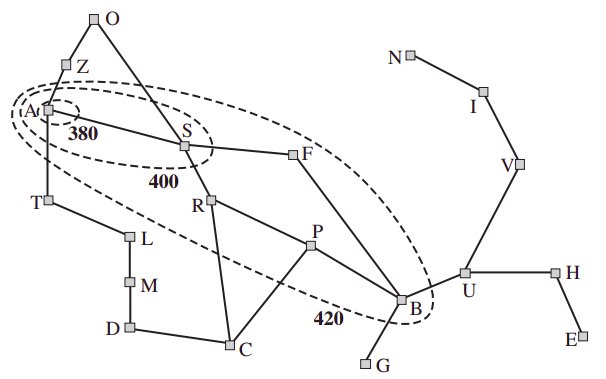
\includegraphics[
        width=\linewidth,
        height=5cm,
        keepaspectratio,
    ]{images/artificial-intelligence/examples/romania-a-star-contours.png}
    \caption*{Nodes inside a given contour have f-costs less than or equal to the contour value. \cite{ai/book/Artificial-Intelligence-A-Modern-Approach/Russell-Norvig}}
\end{figure}

















